\documentclass[11pt]{article}

\usepackage[margin=2.5cm]{geometry}
\usepackage{amsmath,amssymb,amsthm}
\usepackage{booktabs}
\usepackage{graphicx}
\usepackage{mathtools}

\newtheorem{theorem}{Theorem}

\title{Two-Stage Certification Results\\for the GKW Transfer Operator}
\author{}
\date{February 2026}

\begin{document}
\maketitle

% Eigenvalues 1--15: K_low = 48, K_high = 256, N = 5000
% Eigenvalues 16--20: K_low = 64, K_high = 256, N = 5000

\begin{table}[ht]
\centering
\caption{Two-stage certification parameters}
\label{tab:two-stage-params}
\begin{tabular}{ll}
\toprule
Parameter & Value \\
\midrule
$K_{\mathrm{low}}$ & $48$ (eigenvalues $1$--$15$), $64$ (eigenvalues $16$--$20$) \\
$K_{\mathrm{high}}$ & $256$ \\
$C_2$ & $1.005810 \times 10^{1}$ \\
$\varepsilon_{48}$ & $2.366161 \times 10^{-8}$ \\
$\varepsilon_{64}$ & $3.602335 \times 10^{-11}$ \\
$\varepsilon_{256}$ & $5.585504 \times 10^{-45}$ \\
Circle samples & $256$ \\
$N$ (splitting) & $5000$ \\
\bottomrule
\end{tabular}
\end{table}

\begin{table}[ht]
\centering
\caption{Two-stage certification results for the first $20$ eigenvalues of the GKW operator ($s=1$).
The column $\alpha_1 = \varepsilon_{K_{\mathrm{low}}} \cdot \|R_{A_{K_{\mathrm{low}}}}(z)\|$ is the
small-gain factor on the excluding circle $\Gamma_j$.  All $20$ eigenvalues satisfy $\alpha_1 < 1$,
proving simplicity and giving certified resolvent bounds.}
\label{tab:two-stage-results}
\begin{tabular}{rlcccccc}
\toprule
$j$ & $\hat\lambda_j$ & $K_{\mathrm{low}}$ & $\alpha_1$ & Circle $r$ & NK radius & Riesz proj.~error \\
\midrule
1 & $1.0000000000$ & 48 & $1.01 \times 10^{-5}$ & $1.00 \times 10^{-2}$ & $7.40 \times 10^{-45}$ & $1.01 \times 10^{-41}$ \\
2 & $-0.3036630029$ & 48 & $3.53 \times 10^{-5}$ & $3.04 \times 10^{-3}$ & $2.33 \times 10^{-44}$ & $3.77 \times 10^{-41}$ \\
3 & $0.1008845093$ & 48 & $1.11 \times 10^{-4}$ & $1.01 \times 10^{-3}$ & $7.32 \times 10^{-44}$ & $1.23 \times 10^{-40}$ \\
4 & $-0.0354961590$ & 48 & $3.24 \times 10^{-4}$ & $3.55 \times 10^{-4}$ & $2.17 \times 10^{-43}$ & $3.73 \times 10^{-40}$ \\
5 & $0.0128437904$ & 48 & $9.15 \times 10^{-4}$ & $1.28 \times 10^{-4}$ & $6.22 \times 10^{-43}$ & $1.08 \times 10^{-39}$ \\
6 & $-0.0047177775$ & 48 & $2.52 \times 10^{-3}$ & $4.72 \times 10^{-5}$ & $1.75 \times 10^{-42}$ & $3.01 \times 10^{-39}$ \\
7 & $0.0017486751$ & 48 & $6.85 \times 10^{-3}$ & $1.75 \times 10^{-5}$ & $4.85 \times 10^{-42}$ & $8.29 \times 10^{-39}$ \\
8 & $-0.0006520209$ & 48 & $1.84 \times 10^{-2}$ & $6.52 \times 10^{-6}$ & $1.33 \times 10^{-41}$ & $2.29 \times 10^{-38}$ \\
9 & $0.0002441315$ & 48 & $4.91 \times 10^{-2}$ & $2.44 \times 10^{-6}$ & $3.63 \times 10^{-41}$ & $6.49 \times 10^{-38}$ \\
10 & $-0.0000916891$ & 48 & $1.30 \times 10^{-1}$ & $9.17 \times 10^{-7}$ & $9.85 \times 10^{-41}$ & $2.05 \times 10^{-37}$ \\
11 & $0.0000345165$ & 48 & $3.44 \times 10^{-1}$ & $3.45 \times 10^{-7}$ & $2.66 \times 10^{-40}$ & $9.48 \times 10^{-37}$ \\
12 & $-0.0000130177$ & 48 & $4.99 \times 10^{-1}$ & $2.37 \times 10^{-7}$ & $7.16 \times 10^{-40}$ & $2.34 \times 10^{-36}$ \\
13 & $0.0000049168$ & 48 & $4.97 \times 10^{-1}$ & $2.37 \times 10^{-7}$ & $1.92 \times 10^{-39}$ & $2.31 \times 10^{-36}$ \\
14 & $-0.0000018593$ & 48 & $5.01 \times 10^{-1}$ & $2.37 \times 10^{-7}$ & $5.15 \times 10^{-39}$ & $2.38 \times 10^{-36}$ \\
15 & $0.0000007038$ & 48 & $6.21 \times 10^{-1}$ & $2.01 \times 10^{-7}$ & $1.38 \times 10^{-38}$ & $5.36 \times 10^{-36}$ \\
\midrule
16 & $-0.0000002666$ & 64 & $6.86 \times 10^{-2}$ & $2.67 \times 10^{-9}$ & $3.67 \times 10^{-38}$ & $6.22 \times 10^{-35}$ \\
17 & $0.0000001011$ & 64 & $1.80 \times 10^{-1}$ & $1.01 \times 10^{-9}$ & $9.78 \times 10^{-38}$ & $2.09 \times 10^{-34}$ \\
18 & $-0.0000000383$ & 64 & $4.70 \times 10^{-1}$ & $3.84 \times 10^{-10}$ & $2.60 \times 10^{-37}$ & $1.30 \times 10^{-33}$ \\
19 & $0.0000000146$ & 64 & $4.98 \times 10^{-1}$ & $3.60 \times 10^{-10}$ & $6.92 \times 10^{-37}$ & $1.52 \times 10^{-33}$ \\
20 & $-0.0000000055$ & 64 & $4.97 \times 10^{-1}$ & $3.60 \times 10^{-10}$ & $1.84 \times 10^{-36}$ & $1.51 \times 10^{-33}$ \\
\bottomrule
\end{tabular}
\end{table}

\begin{table}[ht]
\centering
\caption{Certified resolvent bounds.  $\|R_{A_{K_{\mathrm{low}}}}\|$ is the resolvent of the
finite-dimensional Galerkin matrix on the excluding circle $\Gamma_j$, certified via
\texttt{run\_certification}.  $M_\infty = \|R_{L_r}(z)\|$ is the certified resolvent bound
for the infinite-dimensional operator, obtained via Neumann perturbation:
$M_\infty \leq \|R_{A_{K_{\mathrm{low}}}}\| / (1 - \alpha_1)$.
The transfer column gives $\|R_{A_{K_{\mathrm{high}}}}\|$ via reverse perturbation
at $K_{\mathrm{high}} = 256$.}
\label{tab:resolvent-bounds}
\begin{tabular}{rlrrrr}
\toprule
$j$ & $K_{\mathrm{low}}$ & $\|R_{A_{K_{\mathrm{low}}}}\|$ & $M_\infty = \|R_{L_r}\|$ & $\alpha_{\mathrm{high}}$ & $\|R_{A_{K_{\mathrm{high}}}}\|$ \\
\midrule
1 & 48 & $4.25 \times 10^{2}$ & $4.25 \times 10^{2}$ & $2.37 \times 10^{-42}$ & $4.25 \times 10^{2}$ \\
2 & 48 & $1.49 \times 10^{3}$ & $1.49 \times 10^{3}$ & $8.33 \times 10^{-42}$ & $1.49 \times 10^{3}$ \\
3 & 48 & $4.67 \times 10^{3}$ & $4.67 \times 10^{3}$ & $2.61 \times 10^{-41}$ & $4.67 \times 10^{3}$ \\
4 & 48 & $1.37 \times 10^{4}$ & $1.37 \times 10^{4}$ & $7.66 \times 10^{-41}$ & $1.37 \times 10^{4}$ \\
5 & 48 & $3.87 \times 10^{4}$ & $3.87 \times 10^{4}$ & $2.16 \times 10^{-40}$ & $3.87 \times 10^{4}$ \\
6 & 48 & $1.07 \times 10^{5}$ & $1.07 \times 10^{5}$ & $5.97 \times 10^{-40}$ & $1.07 \times 10^{5}$ \\
7 & 48 & $2.89 \times 10^{5}$ & $2.91 \times 10^{5}$ & $1.63 \times 10^{-39}$ & $2.91 \times 10^{5}$ \\
8 & 48 & $7.78 \times 10^{5}$ & $7.92 \times 10^{5}$ & $4.43 \times 10^{-39}$ & $7.92 \times 10^{5}$ \\
9 & 48 & $2.07 \times 10^{6}$ & $2.18 \times 10^{6}$ & $1.22 \times 10^{-38}$ & $2.18 \times 10^{6}$ \\
10 & 48 & $5.50 \times 10^{6}$ & $6.33 \times 10^{6}$ & $3.53 \times 10^{-38}$ & $6.33 \times 10^{6}$ \\
11 & 48 & $1.45 \times 10^{7}$ & $2.22 \times 10^{7}$ & $1.24 \times 10^{-37}$ & $2.22 \times 10^{7}$ \\
12 & 48 & $2.11 \times 10^{7}$ & $4.21 \times 10^{7}$ & $2.35 \times 10^{-37}$ & $4.21 \times 10^{7}$ \\
13 & 48 & $2.10 \times 10^{7}$ & $4.18 \times 10^{7}$ & $2.34 \times 10^{-37}$ & $4.18 \times 10^{7}$ \\
14 & 48 & $2.12 \times 10^{7}$ & $4.24 \times 10^{7}$ & $2.37 \times 10^{-37}$ & $4.24 \times 10^{7}$ \\
15 & 48 & $2.62 \times 10^{7}$ & $6.91 \times 10^{7}$ & $3.86 \times 10^{-37}$ & $6.91 \times 10^{7}$ \\
\midrule
16 & 64 & $1.90 \times 10^{9}$ & $2.04 \times 10^{9}$ & $1.14 \times 10^{-35}$ & $2.04 \times 10^{9}$ \\
17 & 64 & $4.99 \times 10^{9}$ & $6.08 \times 10^{9}$ & $3.40 \times 10^{-35}$ & $6.08 \times 10^{9}$ \\
18 & 64 & $1.31 \times 10^{10}$ & $2.47 \times 10^{10}$ & $1.38 \times 10^{-34}$ & $2.47 \times 10^{10}$ \\
19 & 64 & $1.38 \times 10^{10}$ & $2.75 \times 10^{10}$ & $1.54 \times 10^{-34}$ & $2.75 \times 10^{10}$ \\
20 & 64 & $1.38 \times 10^{10}$ & $2.74 \times 10^{10}$ & $1.53 \times 10^{-34}$ & $2.74 \times 10^{10}$ \\
\bottomrule
\end{tabular}
\end{table}

\begin{theorem}[Rigorous spectral certification of the GKW operator]
\label{thm:two-stage}
Let $L_r : H^2(D_r) \to H^2(D_r)$ be the GKW transfer operator for $s=1$,
$r = 1$.  The first $20$ eigenvalues $\lambda_1, \ldots, \lambda_{20}$
(ordered by decreasing modulus) are simple.  For each $j = 1, \ldots, 20$,
there exists a unique $\lambda_j^* \in \sigma(L_r)$ satisfying:
\begin{enumerate}
\item $\lambda_{1}^* \in B(1.000000000000,\; 7.40 \times 10^{-45})$, \quad $\|P_{L_r}(\Gamma_1) - P_{A_{256}}(\Gamma_1)\| \leq 1.01 \times 10^{-41}$
\item $\lambda_{2}^* \in B(-0.303663002899,\; 2.33 \times 10^{-44})$, \quad $\|P_{L_r}(\Gamma_2) - P_{A_{256}}(\Gamma_2)\| \leq 3.77 \times 10^{-41}$
\item $\lambda_{3}^* \in B(0.100884509293,\; 7.32 \times 10^{-44})$, \quad $\|P_{L_r}(\Gamma_3) - P_{A_{256}}(\Gamma_3)\| \leq 1.23 \times 10^{-40}$
\item $\lambda_{4}^* \in B(-0.035496159022,\; 2.17 \times 10^{-43})$, \quad $\|P_{L_r}(\Gamma_4) - P_{A_{256}}(\Gamma_4)\| \leq 3.73 \times 10^{-40}$
\item $\lambda_{5}^* \in B(0.012843790362,\; 6.22 \times 10^{-43})$, \quad $\|P_{L_r}(\Gamma_5) - P_{A_{256}}(\Gamma_5)\| \leq 1.08 \times 10^{-39}$
\item $\lambda_{6}^* \in B(-0.004717777512,\; 1.75 \times 10^{-42})$, \quad $\|P_{L_r}(\Gamma_6) - P_{A_{256}}(\Gamma_6)\| \leq 3.01 \times 10^{-39}$
\item $\lambda_{7}^* \in B(0.001748675124,\; 4.85 \times 10^{-42})$, \quad $\|P_{L_r}(\Gamma_7) - P_{A_{256}}(\Gamma_7)\| \leq 8.29 \times 10^{-39}$
\item $\lambda_{8}^* \in B(-0.000652020858,\; 1.33 \times 10^{-41})$, \quad $\|P_{L_r}(\Gamma_8) - P_{A_{256}}(\Gamma_8)\| \leq 2.29 \times 10^{-38}$
\item $\lambda_{9}^* \in B(0.000244131465,\; 3.63 \times 10^{-41})$, \quad $\|P_{L_r}(\Gamma_9) - P_{A_{256}}(\Gamma_9)\| \leq 6.49 \times 10^{-38}$
\item $\lambda_{10}^* \in B(-0.000091689083,\; 9.85 \times 10^{-41})$, \quad $\|P_{L_r}(\Gamma_{10}) - P_{A_{256}}(\Gamma_{10})\| \leq 2.05 \times 10^{-37}$
\item $\lambda_{11}^* \in B(0.000034516544,\; 2.66 \times 10^{-40})$, \quad $\|P_{L_r}(\Gamma_{11}) - P_{A_{256}}(\Gamma_{11})\| \leq 9.48 \times 10^{-37}$
\item $\lambda_{12}^* \in B(-0.000013017694,\; 7.16 \times 10^{-40})$, \quad $\|P_{L_r}(\Gamma_{12}) - P_{A_{256}}(\Gamma_{12})\| \leq 2.34 \times 10^{-36}$
\item $\lambda_{13}^* \in B(0.000004916774,\; 1.92 \times 10^{-39})$, \quad $\|P_{L_r}(\Gamma_{13}) - P_{A_{256}}(\Gamma_{13})\| \leq 2.31 \times 10^{-36}$
\item $\lambda_{14}^* \in B(-0.000001859292,\; 5.15 \times 10^{-39})$, \quad $\|P_{L_r}(\Gamma_{14}) - P_{A_{256}}(\Gamma_{14})\| \leq 2.38 \times 10^{-36}$
\item $\lambda_{15}^* \in B(0.000000703785,\; 1.38 \times 10^{-38})$, \quad $\|P_{L_r}(\Gamma_{15}) - P_{A_{256}}(\Gamma_{15})\| \leq 5.36 \times 10^{-36}$
\item $\lambda_{16}^* \in B(-0.000000266641,\; 3.67 \times 10^{-38})$, \quad $\|P_{L_r}(\Gamma_{16}) - P_{A_{256}}(\Gamma_{16})\| \leq 6.22 \times 10^{-35}$
\item $\lambda_{17}^* \in B(0.000000101091,\; 9.78 \times 10^{-38})$, \quad $\|P_{L_r}(\Gamma_{17}) - P_{A_{256}}(\Gamma_{17})\| \leq 2.09 \times 10^{-34}$
\item $\lambda_{18}^* \in B(-0.000000038350,\; 2.60 \times 10^{-37})$, \quad $\|P_{L_r}(\Gamma_{18}) - P_{A_{256}}(\Gamma_{18})\| \leq 1.30 \times 10^{-33}$
\item $\lambda_{19}^* \in B(0.000000014556,\; 6.92 \times 10^{-37})$, \quad $\|P_{L_r}(\Gamma_{19}) - P_{A_{256}}(\Gamma_{19})\| \leq 1.52 \times 10^{-33}$
\item $\lambda_{20}^* \in B(-0.000000005528,\; 1.84 \times 10^{-36})$, \quad $\|P_{L_r}(\Gamma_{20}) - P_{A_{256}}(\Gamma_{20})\| \leq 1.51 \times 10^{-33}$
\end{enumerate}
Here $B(c, r)$ denotes the closed ball $\{z \in \mathbb{C} : |z - c| \leq r\}$,
and $\Gamma_j$ is the excluding circle of radius listed in Table~\ref{tab:two-stage-results}
centered at $\hat\lambda_j$.

\medskip\noindent
\textbf{Method.}
Stage~1 certifies that $\Gamma_j \subset \rho(L_r)$ by verifying
$\alpha_1 = \varepsilon_{K_{\mathrm{low}}} \cdot \|R_{A_{K_{\mathrm{low}}}}(z)\|_{(\Gamma_j)} < 1$
via resolvent sampling with $256$ points on $\Gamma_j$, using Galerkin matrices of size
$K_{\mathrm{low}} + 1$ (with $K_{\mathrm{low}} = 48$ for $j = 1, \ldots, 15$ and
$K_{\mathrm{low}} = 64$ for $j = 16, \ldots, 20$).
This yields the certified infinite-dimensional resolvent bound
$M_\infty \coloneqq \|R_{L_r}(z)\|_{(\Gamma_j)} \leq \|R_{A_{K_{\mathrm{low}}}}\| / (1 - \alpha_1)$.
Stage~2 applies a Newton--Kantorovich defect-based argument at $K_{\mathrm{high}} = 256$
($\varepsilon_{256} \approx 5.59 \times 10^{-45}$) to obtain tight eigenpair enclosures.
The Riesz projector error is bounded via
$\|P_{L_r} - P_{A_{K_{\mathrm{high}}}}\| \leq \frac{|\Gamma_j|}{2\pi} \cdot
\frac{\|R_{A_{K_{\mathrm{high}}}}\|^2 \cdot \varepsilon_{K_{\mathrm{high}}}}{1 - \varepsilon_{K_{\mathrm{high}}} \cdot \|R_{A_{K_{\mathrm{high}}}}\|}$,
where $\|R_{A_{K_{\mathrm{high}}}}\|$ is obtained from $M_\infty$ by reverse perturbation.
All scalar bounds use directed rounding to ensure rigor.
\end{theorem}
\clearpage
\section*{Rigorous Spectral Expansion}

Since all $20$ eigenvalues are certified to be simple (Theorem~\ref{thm:two-stage}),
each eigenvalue $\lambda_j$ has a rank-one Riesz projector
$P_j = v_j \otimes \ell_j$,
where $v_j$ is the right eigenvector ($\|v_j\|_2 = 1$) and $\ell_j$ the left (dual) eigenvector,
normalized so that $\ell_j(v_j) = 1$.
The spectral expansion of $L^n$ applied to the constant function $\mathbf{1}$ is
\begin{equation}
\label{eq:spectral-expansion}
L^n \mathbf{1} = \sum_{j=1}^{N} \lambda_j^n \, \ell_j(\mathbf{1}) \, v_j + R_N(n),
\end{equation}
where $\ell_j(\mathbf{1}) = \langle P_j(\mathbf{1}), v_j \rangle$ is the spectral coefficient
and $R_N(n)$ is bounded by $|\lambda_{N+1}|^n$ times the tail projector norm.

\medskip\noindent
\textbf{Computation of $\ell_j(\mathbf{1})$.}
The GKW matrix $A_{256}$ is built in high-precision arithmetic (ArbNumerics, 512 bits)
and rigorously converted to a \texttt{BallMatrix} with BigFloat centers, giving
input uncertainty $\|A_{\mathrm{rad}}\|_2 \leq 5.40 \times 10^{-84}$.
A direct BigFloat Schur decomposition $A = Q T Q'$ is computed via
\texttt{GenericSchur.jl}, achieving residual $\|A - QTQ'\|_2 \leq 2.15 \times 10^{-153}$.
The total Schur enclosure error is
$\|E\| = \|A_{\mathrm{true}} - QTQ'\|_2 \leq 5.40 \times 10^{-84}$.
For each eigenvalue $\lambda_j$, a BigFloat \texttt{ordschur} reorders the target eigenvalue
to position $(1,1)$, and the left eigenvector functional $\ell_j$ is recovered
via Sylvester equation: with $T = \bigl[\begin{smallmatrix} \lambda_j & T_{12} \\ 0 & T_{22}\end{smallmatrix}\bigr]$,
the solution $z_0 = (T_{22} - \lambda_j I)^{-1} w_{\mathrm{rest}}$ gives
$\ell_j(\mathbf{1}) = w_1 - T_{12} \cdot z_0$,
where $w = Q_{1,:}$ is the first row of the reordered~$Q$.
The certified error $\delta$ accounts for the Sylvester residual,
the Schur perturbation $\|E\|$, and the NK eigenvector error:
$\delta \leq \delta_{\mathrm{Sylv}} + \delta_{\mathrm{pert}} + \delta_{\mathrm{NK}}$.
No precision is lost to floating-point conversion; all quantities remain in
512-bit BigFloat arithmetic until the final display.
All $20$ coefficients are certified with $|\ell_j(\mathbf{1})| > \delta$.

\begin{table}[ht]
\centering
\caption{Rigorous spectral expansion coefficients $\ell_j(\mathbf{1})$ at $K = 256$.
Computed via BigFloat Schur decomposition (GenericSchur.jl, 512-bit precision)
with Sylvester-based Riesz projector recovery.
Schur enclosure error $\|E\| \leq 5.40 \times 10^{-84}$.
All $20$ coefficients satisfy $|\ell_j(\mathbf{1})| > \delta$ (sign certified).}
\label{tab:spectral-coefficients}
\begin{tabular}{rllll}
\toprule
$j$ & $\hat\lambda_j$ & $\ell_j(\mathbf{1})$ & $\pm\;\delta$ & $\delta_{\mathrm{pert}}$ \\
\midrule
1 & $1.0000000000$ & $+8.3294037022e-01$ & $1.73e-44$ & $4.24e-83$ \\
2 & $-0.3036630029$ & $+4.5120576837e-01$ & $5.73e-44$ & $3.87e-82$ \\
3 & $0.1008845093$ & $-2.0193987421e-01$ & $1.81e-43$ & $2.79e-81$ \\
4 & $-0.0354961590$ & $+8.7402392976e-02$ & $5.15e-43$ & $1.63e-80$ \\
5 & $0.0128437904$ & $-3.6946161114e-02$ & $1.40e-42$ & $8.44e-80$ \\
6 & $-0.0047177775$ & $+1.5347954161e-02$ & $3.77e-42$ & $4.08e-79$ \\
7 & $0.0017486751$ & $-6.2949804200e-03$ & $1.01e-41$ & $1.90e-78$ \\
8 & $-0.0006520209$ & $+2.5574209148e-03$ & $2.73e-41$ & $8.67e-78$ \\
9 & $0.0002441315$ & $-1.0314151917e-03$ & $7.36e-41$ & $3.94e-77$ \\
10 & $-0.0000916891$ & $+4.1357957447e-04$ & $1.99e-40$ & $1.79e-76$ \\
11 & $0.0000345165$ & $-1.6506736199e-04$ & $5.34e-40$ & $8.10e-76$ \\
12 & $-0.0000130177$ & $+6.5629117564e-05$ & $1.44e-39$ & $3.69e-75$ \\
13 & $0.0000049168$ & $-2.6009716743e-05$ & $3.84e-39$ & $1.68e-74$ \\
14 & $-0.0000018593$ & $+1.0279881381e-05$ & $1.03e-38$ & $7.71e-74$ \\
15 & $0.0000007038$ & $-4.0534029703e-06$ & $2.76e-38$ & $3.54e-73$ \\
16 & $-0.0000002666$ & $+1.5950118399e-06$ & $7.34e-38$ & $1.63e-72$ \\
17 & $0.0000001011$ & $-6.2651170652e-07$ & $1.96e-37$ & $7.54e-72$ \\
18 & $-0.0000000383$ & $+2.4570015817e-07$ & $5.20e-37$ & $3.49e-71$ \\
19 & $0.0000000146$ & $-9.6220523878e-08$ & $1.38e-36$ & $1.62e-70$ \\
20 & $-0.0000000055$ & $+3.7633916395e-08$ & $3.68e-36$ & $7.52e-70$ \\
\bottomrule
\end{tabular}
\end{table}
\clearpage
\subsection*{Eigenfunctions}

The following figures show the eigenfunctions $v_j(x)$ evaluated on $[0.01, 0.99]$
in the shifted monomial basis $\{(x-1)^k\}_{k=0}^{K}$, with $K = 256$.

\begin{figure}[ht]
\centering
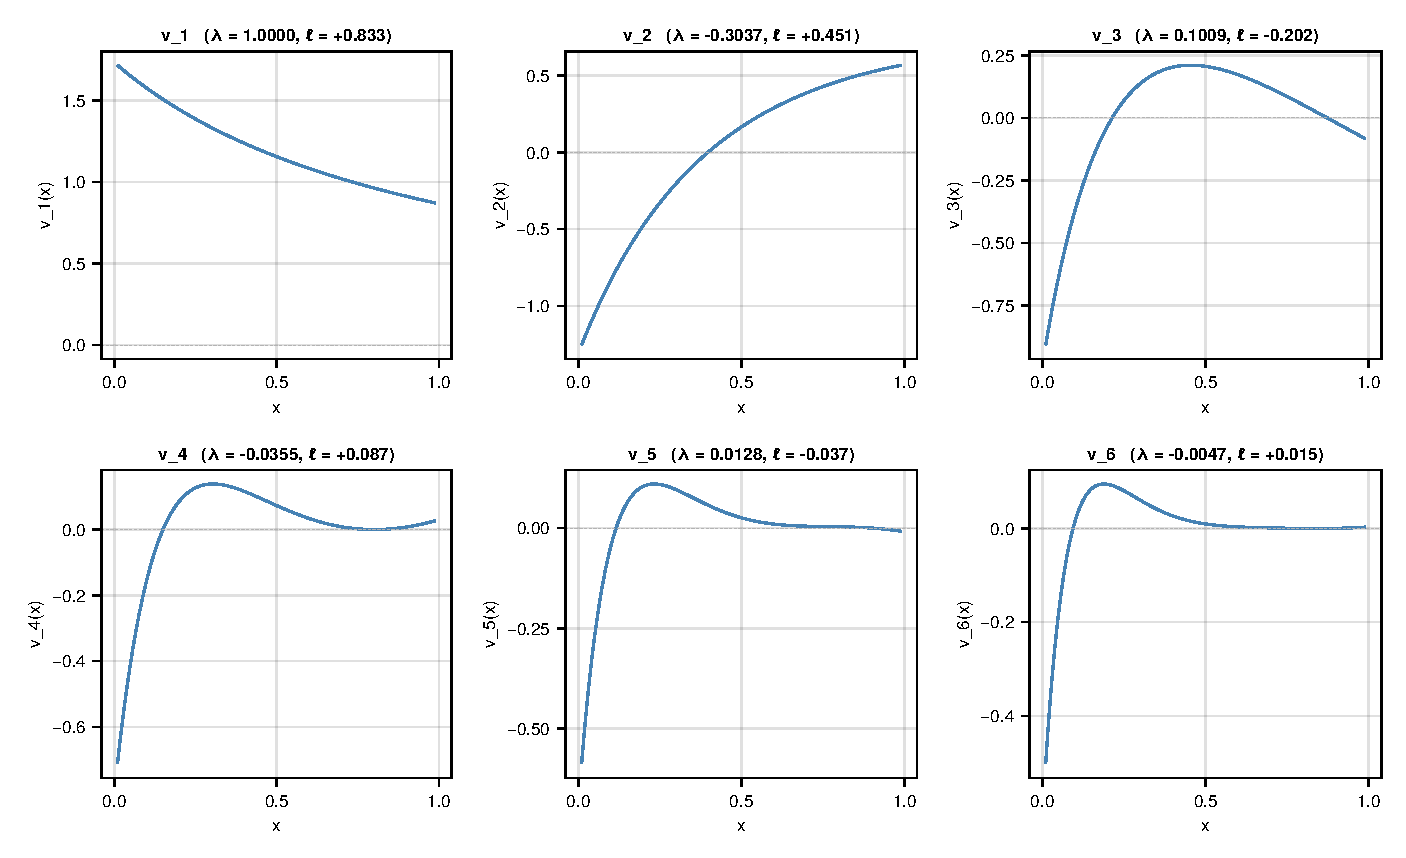
\includegraphics[width=\textwidth]{eigenfunctions_1_6.pdf}
\caption{Leading eigenfunctions $v_1, \ldots, v_6$. The invariant density $v_1$ (top left)
is positive; higher eigenfunctions oscillate with increasing frequency.
Each panel shows $\lambda_j$ and $\ell_j(\mathbf{1})$.}
\label{fig:eigenfunctions-1-6}
\end{figure}

\begin{figure}[ht]
\centering
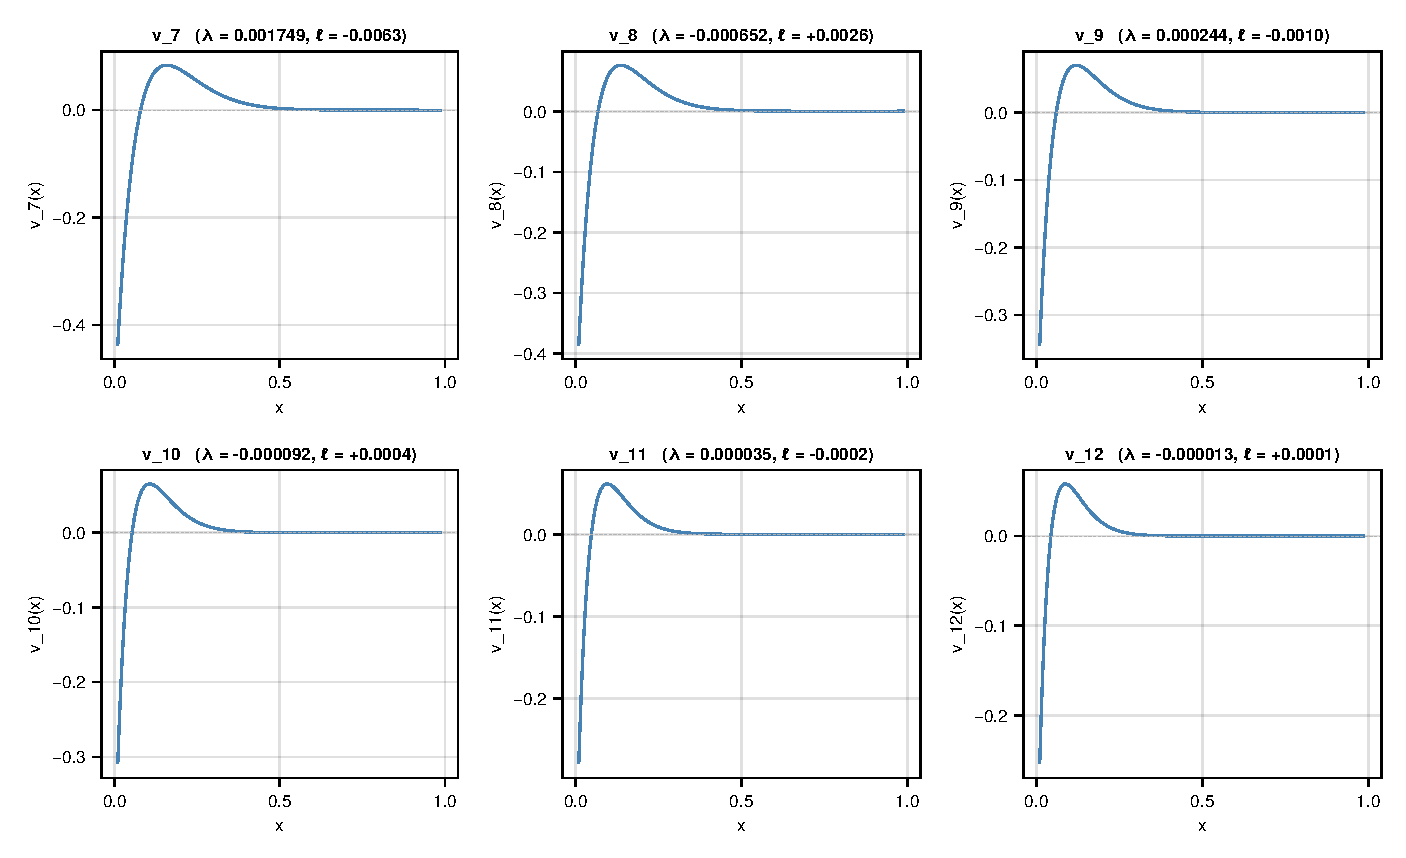
\includegraphics[width=\textwidth]{eigenfunctions_7_12.pdf}
\caption{Higher eigenfunctions $v_7, \ldots, v_{12}$.
The corresponding eigenvalues $|\lambda_j|$ are of order $10^{-3}$--$10^{-5}$;
these modes decay rapidly under iteration.}
\label{fig:eigenfunctions-7-12}
\end{figure}

\begin{figure}[ht]
\centering
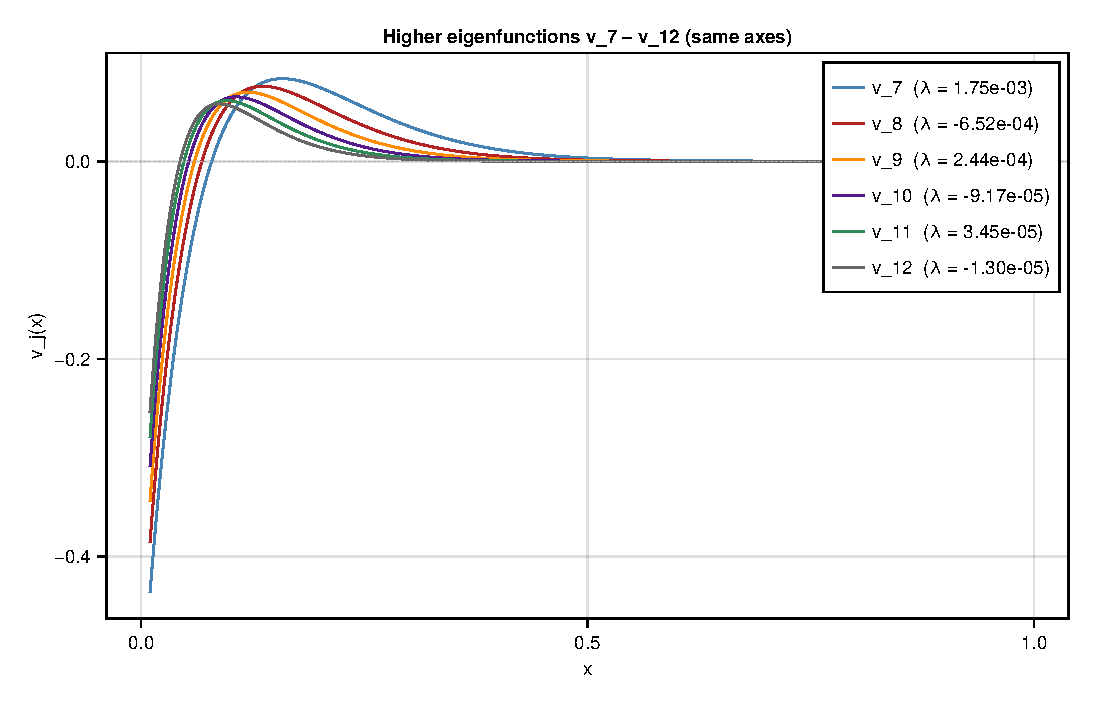
\includegraphics[width=0.85\textwidth]{eigenfunctions_7_12_overlay.pdf}
\caption{Higher eigenfunctions $v_7, \ldots, v_{12}$ overlaid on the same axes,
showing their relative magnitudes and the progressive decay of amplitude with
increasing index.}
\label{fig:eigenfunctions-7-12-overlay}
\end{figure}

\begin{figure}[ht]
\centering
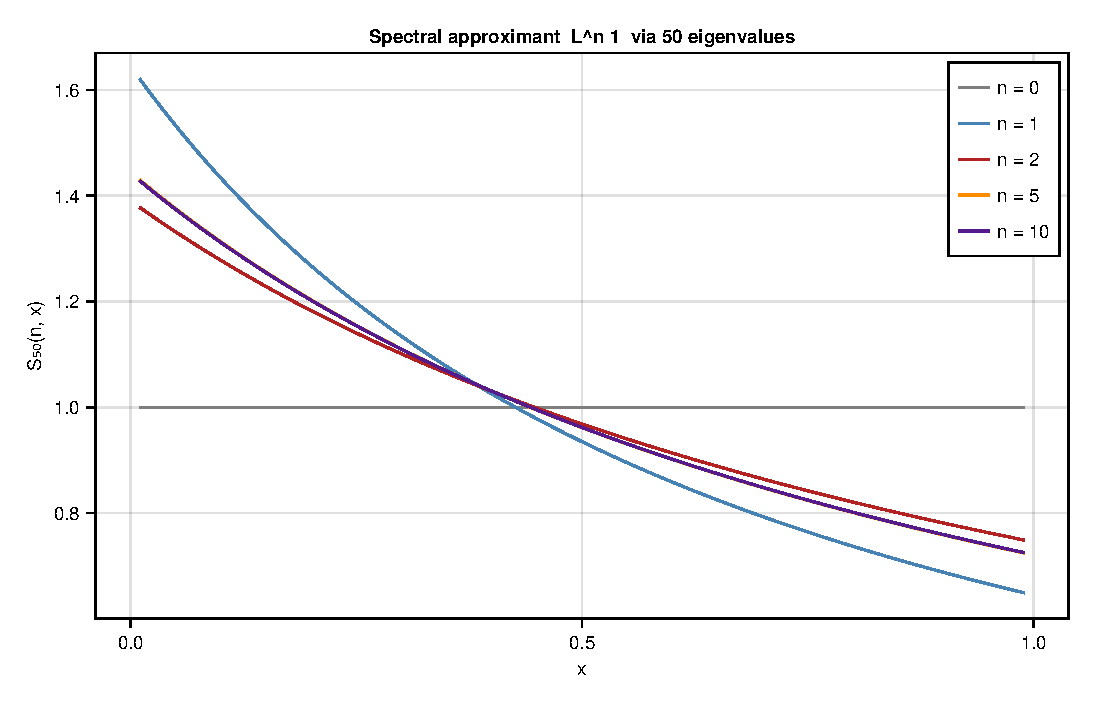
\includegraphics[width=0.85\textwidth]{spectral_approximant.pdf}
\caption{Spectral approximant $S_{20}(n, x) = \sum_{j=1}^{20} \lambda_j^n \, \ell_j(\mathbf{1}) \, v_j(x)$
for $n = 0, 1, 2, 5, 10$.  At $n = 0$ the sum reconstructs the constant function~$\mathbf{1}$;
at $n = 1$ it approximates the transfer operator applied to~$\mathbf{1}$;
for large~$n$ it converges to $\lambda_1^n \, \ell_1(\mathbf{1}) \, v_1(x)$.}
\label{fig:spectral-approximant}
\end{figure}

\begin{figure}[ht]
\centering
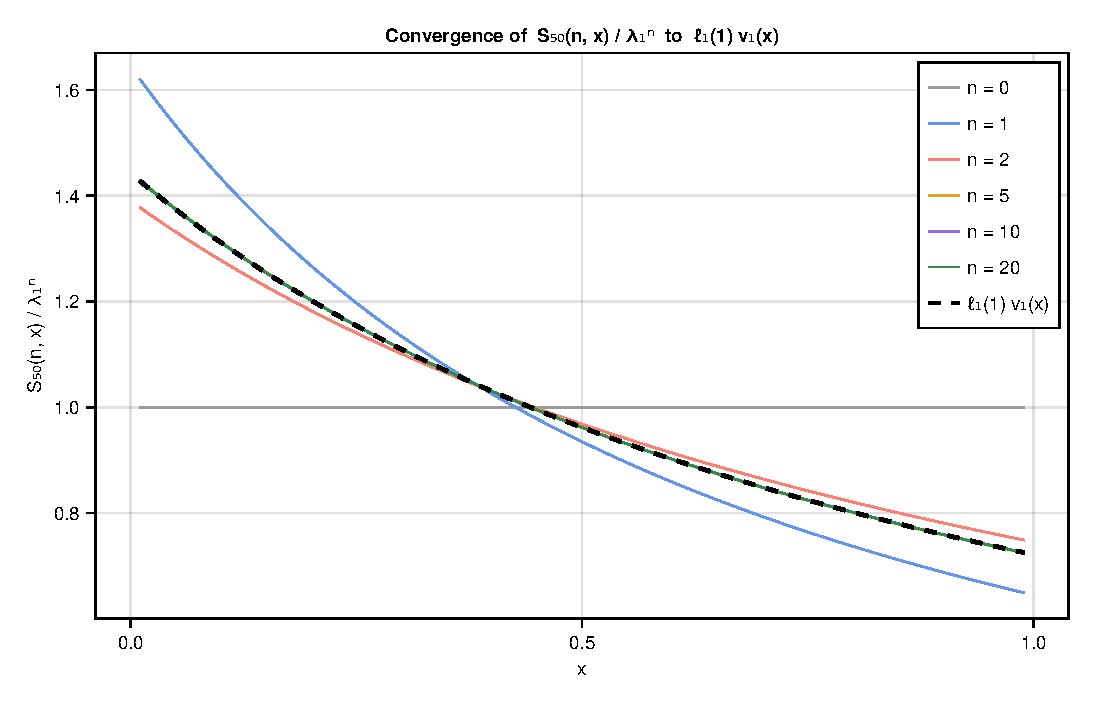
\includegraphics[width=0.85\textwidth]{spectral_convergence.pdf}
\caption{Convergence of $S_{20}(n, x) / \lambda_1^n$ to the invariant density
$\ell_1(\mathbf{1}) \, v_1(x)$ (dashed black).
The spectral gap $|\lambda_2 / \lambda_1| \approx 0.304$ governs the rate of convergence.}
\label{fig:spectral-convergence}
\end{figure}

\clearpage
\subsection*{Eigenvector Coefficients $[v_j]_k$}

The following tables list the first $50$ coefficients of each unit-norm
eigenvector $v_j$ in the shifted monomial basis $\{(w-1)^k\}_{k=0}^{K}$.
Each coefficient is known to within $\pm\, r_{\mathrm{NK}}$
(Table~\ref{tab:two-stage-results}), where $r_{\mathrm{NK}}$
is the Newton--Kantorovich eigenpair enclosure radius;
the $\ell^2$ error $\|\hat{v}_j - v_j\|_2 \leq r_{\mathrm{NK}}$
is shown for each eigenvector.

\paragraph{$j = 1$: $\lambda_{1} = 1.000000e+00$, \quad $\ell_{1}(\mathbf{1}) = +8.329404e{-}01$, \quad $\|\hat{v}_1 - v_1\|_2 \leq 7.40e{-}45$}
\begin{center}
{\footnotesize
\begin{tabular}{r@{\;\;}l@{\quad}r@{\;\;}l}
\toprule
$k$ & $[v_{1}]_k$ & $k$ & $[v_{1}]_k$ \\
\midrule
0 & $+8.6602540378e-01$ & 25 & $-2.5809568280e-08$ \\
1 & $-4.3301270189e-01$ & 26 & $+1.2904784140e-08$ \\
2 & $+2.1650635095e-01$ & 27 & $-6.4523920699e-09$ \\
3 & $-1.0825317547e-01$ & 28 & $+3.2261960349e-09$ \\
4 & $+5.4126587737e-02$ & 29 & $-1.6130980175e-09$ \\
5 & $-2.7063293868e-02$ & 30 & $+8.0654900873e-10$ \\
6 & $+1.3531646934e-02$ & 31 & $-4.0327450437e-10$ \\
7 & $-6.7658234671e-03$ & 32 & $+2.0163725218e-10$ \\
8 & $+3.3829117335e-03$ & 33 & $-1.0081862609e-10$ \\
9 & $-1.6914558668e-03$ & 34 & $+5.0409313046e-11$ \\
10 & $+8.4572793338e-04$ & 35 & $-2.5204656523e-11$ \\
11 & $-4.2286396669e-04$ & 36 & $+1.2602328261e-11$ \\
12 & $+2.1143198335e-04$ & 37 & $-6.3011641307e-12$ \\
13 & $-1.0571599167e-04$ & 38 & $+3.1505820654e-12$ \\
14 & $+5.2857995836e-05$ & 39 & $-1.5752910327e-12$ \\
15 & $-2.6428997918e-05$ & 40 & $+7.8764551634e-13$ \\
16 & $+1.3214498959e-05$ & 41 & $-3.9382275817e-13$ \\
17 & $-6.6072494796e-06$ & 42 & $+1.9691137909e-13$ \\
18 & $+3.3036247398e-06$ & 43 & $-9.8455689543e-14$ \\
19 & $-1.6518123699e-06$ & 44 & $+4.9227844771e-14$ \\
20 & $+8.2590618494e-07$ & 45 & $-2.4613922386e-14$ \\
21 & $-4.1295309247e-07$ & 46 & $+1.2306961193e-14$ \\
22 & $+2.0647654624e-07$ & 47 & $-6.1534805964e-15$ \\
23 & $-1.0323827312e-07$ & 48 & $+3.0767402982e-15$ \\
24 & $+5.1619136559e-08$ & 49 & $-1.5383701491e-15$ \\
\bottomrule
\end{tabular}
}
\end{center}

\paragraph{$j = 2$: $\lambda_{2} = -3.036630e{-}01$, \quad $\ell_{2}(\mathbf{1}) = +4.512058e{-}01$, \quad $\|\hat{v}_2 - v_2\|_2 \leq 2.33e{-}44$}
\begin{center}
{\footnotesize
\begin{tabular}{r@{\;\;}l@{\quad}r@{\;\;}l}
\toprule
$k$ & $[v_{2}]_k$ & $k$ & $[v_{2}]_k$ \\
\midrule
0 & $+5.7050920659e-01$ & 25 & $+2.1137822436e-07$ \\
1 & $+4.1624549960e-01$ & 26 & $-1.0569761625e-07$ \\
2 & $-5.1196167436e-01$ & 27 & $+5.2851197768e-08$ \\
3 & $+3.8491986254e-01$ & 28 & $-2.6426213142e-08$ \\
4 & $-2.4616997141e-01$ & 29 & $+1.3213239926e-08$ \\
5 & $+1.4508248976e-01$ & 30 & $-6.6066375954e-09$ \\
6 & $-8.1412161204e-02$ & 31 & $+3.3033150334e-09$ \\
7 & $+4.4232939695e-02$ & 32 & $-1.6516529702e-09$ \\
8 & $-2.3500357920e-02$ & 33 & $+8.2582392107e-10$ \\
9 & $+1.2286594354e-02$ & 34 & $-4.1291080660e-10$ \\
10 & $-6.3488447731e-03$ & 35 & $+2.0645495059e-10$ \\
11 & $+3.2523318873e-03$ & 36 & $-1.0322731864e-10$ \\
12 & $-1.6553890182e-03$ & 37 & $+5.1613613481e-11$ \\
13 & $+8.3854489512e-04$ & 38 & $-2.5806797425e-11$ \\
14 & $-4.2326095063e-04$ & 39 & $+1.2903399301e-11$ \\
15 & $+2.1308196815e-04$ & 40 & $-6.4517018099e-12$ \\
16 & $-1.0706384161e-04$ & 41 & $+3.2258525849e-12$ \\
17 & $+5.3718283692e-05$ & 42 & $-1.6129272967e-12$ \\
18 & $-2.6924831316e-05$ & 43 & $+8.0646418026e-13$ \\
19 & $+1.3485294563e-05$ & 44 & $-4.0323235203e-13$ \\
20 & $-6.7505119961e-06$ & 45 & $+2.0161629853e-13$ \\
21 & $+3.3779201786e-06$ & 46 & $-1.0080820435e-13$ \\
22 & $-1.6898475614e-06$ & 47 & $+5.0404126138e-14$ \\
23 & $+8.4521363390e-07$ & 48 & $-2.5202073187e-14$ \\
24 & $-4.2269924754e-07$ & 49 & $+1.2601040747e-14$ \\
\bottomrule
\end{tabular}
}
\end{center}

\paragraph{$j = 3$: $\lambda_{3} = 1.008845e{-}01$, \quad $\ell_{3}(\mathbf{1}) = -2.019399e{-}01$, \quad $\|\hat{v}_3 - v_3\|_2 \leq 7.32e{-}44$}
\begin{center}
{\footnotesize
\begin{tabular}{r@{\;\;}l@{\quad}r@{\;\;}l}
\toprule
$k$ & $[v_{3}]_k$ & $k$ & $[v_{3}]_k$ \\
\midrule
0 & $-9.0447344941e-02$ & 25 & $+1.4405034690e-06$ \\
1 & $-7.0686601071e-01$ & 26 & $-7.2111182399e-07$ \\
2 & $+9.4489856788e-02$ & 27 & $+3.6084832338e-07$ \\
3 & $+3.0867750376e-01$ & 28 & $-1.8052087863e-07$ \\
4 & $-4.0512541768e-01$ & 29 & $+9.0291304149e-08$ \\
5 & $+3.4761664596e-01$ & 30 & $-4.5155022432e-08$ \\
6 & $-2.4964571405e-01$ & 31 & $+2.2580145600e-08$ \\
7 & $+1.6202173376e-01$ & 32 & $-1.1290716982e-08$ \\
8 & $-9.8450913170e-02$ & 33 & $+5.6454685428e-09$ \\
9 & $+5.7125257848e-02$ & 34 & $-2.8227263359e-09$ \\
10 & $-3.2043727636e-02$ & 35 & $+1.4113422414e-09$ \\
11 & $+1.7521112776e-02$ & 36 & $-7.0565691808e-10$ \\
12 & $-9.3937359563e-03$ & 37 & $+3.5282096728e-10$ \\
13 & $+4.9597294662e-03$ & 38 & $-1.7640697401e-10$ \\
14 & $-2.5873265244e-03$ & 39 & $+8.8201962240e-11$ \\
15 & $+1.3369832382e-03$ & 40 & $-4.4100355916e-11$ \\
16 & $-6.8572831237e-04$ & 41 & $+2.2049934531e-11$ \\
17 & $+3.4963821569e-04$ & 42 & $-1.1024877405e-11$ \\
18 & $-1.7744974958e-04$ & 43 & $+5.5124075668e-12$ \\
19 & $+8.9734547254e-05$ & 44 & $-2.7561939091e-12$ \\
20 & $-4.5250271856e-05$ & 45 & $+1.3780942688e-12$ \\
21 & $+2.2768685168e-05$ & 46 & $-6.8904664447e-13$ \\
22 & $-1.1437476432e-05$ & 47 & $+3.4452338541e-13$ \\
23 & $+5.7381449931e-06$ & 48 & $-1.7226182909e-13$ \\
24 & $-2.8760584487e-06$ & 49 & $+8.6131015376e-14$ \\
\bottomrule
\end{tabular}
}
\end{center}

\paragraph{$j = 4$: $\lambda_{4} = -3.549616e{-}02$, \quad $\ell_{4}(\mathbf{1}) = +8.740239e{-}02$, \quad $\|\hat{v}_4 - v_4\|_2 \leq 2.17e{-}43$}
\begin{center}
{\footnotesize
\begin{tabular}{r@{\;\;}l@{\quad}r@{\;\;}l}
\toprule
$k$ & $[v_{4}]_k$ & $k$ & $[v_{4}]_k$ \\
\midrule
0 & $+2.9668451307e-02$ & 25 & $+9.3012438559e-06$ \\
1 & $+2.7924054265e-01$ & 26 & $-4.6825960255e-06$ \\
2 & $+5.6853860189e-01$ & 27 & $+2.3534773267e-06$ \\
3 & $-4.4824188327e-01$ & 28 & $-1.1813144791e-06$ \\
4 & $+3.3409474574e-02$ & 29 & $+5.9235060337e-07$ \\
5 & $+2.5167800897e-01$ & 30 & $-2.9679138185e-07$ \\
6 & $-3.4618786849e-01$ & 31 & $+1.4861544706e-07$ \\
7 & $+3.2023977666e-01$ & 32 & $-7.4384269422e-08$ \\
8 & $-2.4757279345e-01$ & 33 & $+3.7218012651e-08$ \\
9 & $+1.7190363582e-01$ & 34 & $-1.8617414047e-08$ \\
10 & $-1.1098770133e-01$ & 35 & $+9.3112868289e-09$ \\
11 & $+6.7973144203e-02$ & 36 & $-4.6563649096e-09$ \\
12 & $-3.9996876950e-02$ & 37 & $+2.3283501234e-09$ \\
13 & $+2.2812107298e-02$ & 38 & $-1.1641958726e-09$ \\
14 & $-1.2691930309e-02$ & 39 & $+5.8208892068e-10$ \\
15 & $+6.9215101502e-03$ & 40 & $-2.9103450369e-10$ \\
16 & $-3.7136745268e-03$ & 41 & $+1.4551100833e-10$ \\
17 & $+1.9661656212e-03$ & 42 & $-7.2752230647e-11$ \\
18 & $-1.0296382006e-03$ & 43 & $+3.6374552655e-11$ \\
19 & $+5.3437088712e-04$ & 44 & $-1.8186574860e-11$ \\
20 & $-2.7529049710e-04$ & 45 & $+9.0929869113e-12$ \\
21 & $+1.4096381725e-04$ & 46 & $-4.5463697302e-12$ \\
22 & $-7.1824532168e-05$ & 47 & $+2.2731358030e-12$ \\
23 & $+3.6449132229e-05$ & 48 & $-1.1365491915e-12$ \\
24 & $-1.8436745987e-05$ & 49 & $+5.6826777399e-13$ \\
\bottomrule
\end{tabular}
}
\end{center}

\paragraph{$j = 5$: $\lambda_{5} = 1.284379e{-}02$, \quad $\ell_{5}(\mathbf{1}) = -3.694616e{-}02$, \quad $\|\hat{v}_5 - v_5\|_2 \leq 6.22e{-}43$}
\begin{center}
{\footnotesize
\begin{tabular}{r@{\;\;}l@{\quad}r@{\;\;}l}
\toprule
$k$ & $[v_{5}]_k$ & $k$ & $[v_{5}]_k$ \\
\midrule
0 & $-8.8043043986e-03$ & 25 & $+5.6712684176e-05$ \\
1 & $-1.2821141655e-01$ & 26 & $-2.8984255395e-05$ \\
2 & $-4.0620172038e-01$ & 27 & $+1.4751250734e-05$ \\
3 & $-2.5046189333e-01$ & 28 & $-7.4813774835e-06$ \\
4 & $+5.3864569107e-01$ & 29 & $+3.7833678490e-06$ \\
5 & $-3.4385788333e-01$ & 30 & $-1.9087125191e-06$ \\
6 & $+1.7687881189e-02$ & 31 & $+9.6107039237e-07$ \\
7 & $+2.1476374450e-01$ & 32 & $-4.8314951109e-07$ \\
8 & $-3.0753683353e-01$ & 33 & $+2.4257905525e-07$ \\
9 & $+3.0005617346e-01$ & 34 & $-1.2166964329e-07$ \\
10 & $-2.4487939302e-01$ & 35 & $+6.0976298735e-08$ \\
11 & $+1.7911864358e-01$ & 36 & $-3.0539790507e-08$ \\
12 & $-1.2144537659e-01$ & 37 & $+1.5288308267e-08$ \\
13 & $+7.7837988391e-02$ & 38 & $-7.6505288082e-09$ \\
14 & $-4.7763889976e-02$ & 39 & $+3.8273865267e-09$ \\
15 & $+2.8311025326e-02$ & 40 & $-1.9143609935e-09$ \\
16 & $-1.6314781544e-02$ & 41 & $+9.5737228056e-10$ \\
17 & $+9.1859688538e-03$ & 42 & $-4.7873208370e-10$ \\
18 & $-5.0730711145e-03$ & 43 & $+2.3937206451e-10$ \\
19 & $+2.7565802706e-03$ & 44 & $-1.1968356974e-10$ \\
20 & $-1.4775041526e-03$ & 45 & $+5.9838916142e-11$ \\
21 & $+7.8281931439e-04$ & 46 & $-2.9917598054e-11$ \\
22 & $-4.1071277215e-04$ & 47 & $+1.4957792419e-11$ \\
23 & $+2.1370271470e-04$ & 48 & $-7.4783998741e-12$ \\
24 & $-1.1041605544e-04$ & 49 & $+3.7389693930e-12$ \\
\bottomrule
\end{tabular}
}
\end{center}

\paragraph{$j = 6$: $\lambda_{6} = -4.717778e{-}03$, \quad $\ell_{6}(\mathbf{1}) = +1.534795e{-}02$, \quad $\|\hat{v}_6 - v_6\|_2 \leq 1.75e{-}42$}
\begin{center}
{\footnotesize
\begin{tabular}{r@{\;\;}l@{\quad}r@{\;\;}l}
\toprule
$k$ & $[v_{6}]_k$ & $k$ & $[v_{6}]_k$ \\
\midrule
0 & $+2.9288005304e-03$ & 25 & $+3.1381308619e-04$ \\
1 & $+5.2713511483e-02$ & 26 & $-1.6480576749e-04$ \\
2 & $+2.5758421280e-01$ & 27 & $+8.5893432199e-05$ \\
3 & $+3.7733209909e-01$ & 28 & $-4.4471579252e-05$ \\
4 & $-8.7332643623e-02$ & 29 & $+2.2894637725e-05$ \\
5 & $-3.7954659177e-01$ & 30 & $-1.1728959324e-05$ \\
6 & $+4.8680576276e-01$ & 31 & $+5.9836173338e-06$ \\
7 & $-2.8921038250e-01$ & 32 & $-3.0416841901e-06$ \\
8 & $+1.4754988883e-02$ & 33 & $+1.5415053684e-06$ \\
9 & $+1.8736691367e-01$ & 34 & $-7.7922335306e-07$ \\
10 & $-2.7901534902e-01$ & 35 & $+3.9304657578e-07$ \\
11 & $+2.8413322669e-01$ & 36 & $-1.9790044778e-07$ \\
12 & $-2.4217035435e-01$ & 37 & $+9.9495772191e-08$ \\
13 & $+1.8484043104e-01$ & 38 & $-4.9961213509e-08$ \\
14 & $-1.3057138188e-01$ & 39 & $+2.5062840942e-08$ \\
15 & $+8.7022433528e-02$ & 40 & $-1.2562613434e-08$ \\
16 & $-5.5410631501e-02$ & 41 & $+6.2929196399e-09$ \\
17 & $+3.4005412572e-02$ & 42 & $-3.1506873855e-09$ \\
18 & $-2.0244519606e-02$ & 43 & $+1.5768401622e-09$ \\
19 & $+1.1749626794e-02$ & 44 & $-7.8893057108e-10$ \\
20 & $-6.6741449169e-03$ & 45 & $+3.9463051949e-10$ \\
21 & $+3.7221436445e-03$ & 46 & $-1.9736447204e-10$ \\
22 & $-2.0433607145e-03$ & 47 & $+9.8694741850e-11$ \\
23 & $+1.1066109468e-03$ & 48 & $-4.9349373601e-11$ \\
24 & $-5.9230063610e-04$ & 49 & $+2.4674256052e-11$ \\
\bottomrule
\end{tabular}
}
\end{center}

\paragraph{$j = 7$: $\lambda_{7} = 1.748675e{-}03$, \quad $\ell_{7}(\mathbf{1}) = -6.294980e{-}03$, \quad $\|\hat{v}_7 - v_7\|_2 \leq 4.85e{-}42$}
\begin{center}
{\footnotesize
\begin{tabular}{r@{\;\;}l@{\quad}r@{\;\;}l}
\toprule
$k$ & $[v_{7}]_k$ & $k$ & $[v_{7}]_k$ \\
\midrule
0 & $-9.8055287385e-04$ & 25 & $+1.5153807365e-03$ \\
1 & $-2.1860588173e-02$ & 26 & $-8.2791609363e-04$ \\
2 & $-1.3820176619e-01$ & 27 & $+4.4707439112e-04$ \\
3 & $-3.4256938976e-01$ & 28 & $-2.3895005724e-04$ \\
4 & $-1.9744018209e-01$ & 29 & $+1.2656057412e-04$ \\
5 & $+2.9440585261e-01$ & 30 & $-6.6499936385e-05$ \\
6 & $+8.8207678372e-02$ & 31 & $+3.4696854350e-05$ \\
7 & $-4.1415744698e-01$ & 32 & $-1.7991781746e-05$ \\
8 & $+4.4439275024e-01$ & 33 & $+9.2790396749e-06$ \\
9 & $-2.5719478485e-01$ & 34 & $-4.7629002568e-06$ \\
10 & $+1.7193970567e-02$ & 35 & $+2.4346886257e-06$ \\
11 & $+1.6505458952e-01$ & 36 & $-1.2400950839e-06$ \\
12 & $-2.5611455673e-01$ & 37 & $+6.2967608130e-07$ \\
13 & $+2.7071961776e-01$ & 38 & $-3.1887337166e-07$ \\
14 & $-2.3939660325e-01$ & 39 & $+1.6111110867e-07$ \\
15 & $+1.8947230843e-01$ & 40 & $-8.1243217250e-08$ \\
16 & $-1.3866088775e-01$ & 41 & $+4.0900992244e-08$ \\
17 & $+9.5628348606e-02$ & 42 & $-2.0562710360e-08$ \\
18 & $-6.2923782054e-02$ & 43 & $+1.0325871095e-08$ \\
19 & $+3.9847890015e-02$ & 44 & $-5.1803558743e-09$ \\
20 & $-2.4442242880e-02$ & 45 & $+2.5968910133e-09$ \\
21 & $+1.4593481152e-02$ & 46 & $-1.3009868701e-09$ \\
22 & $-8.5143110135e-03$ & 47 & $+6.5143531766e-10$ \\
23 & $+4.8694811257e-03$ & 48 & $-3.2605766463e-10$ \\
24 & $-2.7370962618e-03$ & 49 & $+1.6314741925e-10$ \\
\bottomrule
\end{tabular}
}
\end{center}

\paragraph{$j = 8$: $\lambda_{8} = -6.520209e{-}04$, \quad $\ell_{8}(\mathbf{1}) = +2.557421e{-}03$, \quad $\|\hat{v}_8 - v_8\|_2 \leq 1.33e{-}41$}
\begin{center}
{\footnotesize
\begin{tabular}{r@{\;\;}l@{\quad}r@{\;\;}l}
\toprule
$k$ & $[v_{8}]_k$ & $k$ & $[v_{8}]_k$ \\
\midrule
0 & $+3.3816038721e-04$ & 25 & $+6.2014947319e-03$ \\
1 & $+8.8712621469e-03$ & 26 & $-3.5661271091e-03$ \\
2 & $+7.0040265312e-02$ & 27 & $+2.0174580968e-03$ \\
3 & $+2.3725221109e-01$ & 28 & $-1.1249354472e-03$ \\
4 & $+3.2135236940e-01$ & 29 & $+6.1924650269e-04$ \\
5 & $-4.5408229903e-02$ & 30 & $-3.3699277531e-04$ \\
6 & $-2.9898964426e-01$ & 31 & $+1.8152382819e-04$ \\
7 & $+1.7562043210e-01$ & 32 & $-9.6889519810e-05$ \\
8 & $+1.8249405818e-01$ & 33 & $+5.1294747872e-05$ \\
9 & $-4.1882715750e-01$ & 34 & $-2.6958830190e-05$ \\
10 & $+4.1193080144e-01$ & 35 & $+1.4076757346e-05$ \\
11 & $-2.3751440328e-01$ & 36 & $-7.3077905994e-06$ \\
12 & $+2.2412015993e-02$ & 37 & $+3.7742513570e-06$ \\
13 & $+1.4574225898e-01$ & 38 & $-1.9403952820e-06$ \\
14 & $-2.3660112868e-01$ & 39 & $+9.9356040970e-07$ \\
15 & $+2.5882669856e-01$ & 40 & $-5.0693439770e-07$ \\
16 & $-2.3645950137e-01$ & 41 & $+2.5784095463e-07$ \\
17 & $+1.9320544604e-01$ & 42 & $-1.3078741619e-07$ \\
18 & $-1.4587027901e-01$ & 43 & $+6.6183319911e-08$ \\
19 & $+1.0370377154e-01$ & 44 & $-3.3422489643e-08$ \\
20 & $-7.0278596440e-02$ & 45 & $+1.6848507392e-08$ \\
21 & $+4.5790881619e-02$ & 46 & $-8.4806233509e-09$ \\
22 & $-2.8867930402e-02$ & 47 & $+4.2632096248e-09$ \\
23 & $+1.7694940545e-02$ & 48 & $-2.1407970004e-09$ \\
24 & $-1.0586583669e-02$ & 49 & $+1.0740409385e-09$ \\
\bottomrule
\end{tabular}
}
\end{center}

\paragraph{$j = 9$: $\lambda_{9} = 2.441315e{-}04$, \quad $\ell_{9}(\mathbf{1}) = -1.031415e{-}03$, \quad $\|\hat{v}_9 - v_9\|_2 \leq 3.63e{-}41$}
\begin{center}
{\footnotesize
\begin{tabular}{r@{\;\;}l@{\quad}r@{\;\;}l}
\toprule
$k$ & $[v_{9}]_k$ & $k$ & $[v_{9}]_k$ \\
\midrule
0 & $-1.1799547910e-04$ & 25 & $+2.1031142393e-02$ \\
1 & $-3.5825018552e-03$ & 26 & $-1.2881889170e-02$ \\
2 & $-3.3725281451e-02$ & 27 & $+7.7187224649e-03$ \\
3 & $-1.4603058030e-01$ & 28 & $-4.5360503861e-03$ \\
4 & $-2.9886824515e-01$ & 29 & $+2.6200998185e-03$ \\
5 & $-1.8545475471e-01$ & 30 & $-1.4902832301e-03$ \\
6 & $+2.3247141884e-01$ & 31 & $+8.3603637339e-04$ \\
7 & $+1.3477449923e-01$ & 32 & $-4.6322633391e-04$ \\
8 & $-2.8813177543e-01$ & 33 & $+2.5380915511e-04$ \\
9 & $+8.1173431804e-02$ & 34 & $-1.3767079278e-04$ \\
10 & $+2.3449479102e-01$ & 35 & $+7.3998208039e-05$ \\
11 & $-4.1289479127e-01$ & 36 & $-3.9448207702e-05$ \\
12 & $+3.8721655110e-01$ & 37 & $+2.0873984602e-05$ \\
13 & $-2.2531195759e-01$ & 38 & $-1.0971579021e-05$ \\
14 & $+2.9238457729e-02$ & 39 & $+5.7319787919e-06$ \\
15 & $+1.2834557148e-01$ & 40 & $-2.9783320709e-06$ \\
16 & $-2.1925984696e-01$ & 41 & $+1.5399771601e-06$ \\
17 & $+2.4787497215e-01$ & 42 & $-7.9277105056e-07$ \\
18 & $-2.3328565645e-01$ & 43 & $+4.0651382364e-07$ \\
19 & $+1.9615236620e-01$ & 44 & $-2.0772176822e-07$ \\
20 & $-1.5229855765e-01$ & 45 & $+1.0581266317e-07$ \\
21 & $+1.1127777959e-01$ & 46 & $-5.3752382090e-08$ \\
22 & $-7.7451963565e-02$ & 47 & $+2.7239826076e-08$ \\
23 & $+5.1792687547e-02$ & 48 & $-1.3774854450e-08$ \\
24 & $-3.3484691285e-02$ & 49 & $+6.9528595371e-09$ \\
\bottomrule
\end{tabular}
}
\end{center}

\paragraph{$j = 10$: $\lambda_{10} = -9.168908e{-}05$, \quad $\ell_{10}(\mathbf{1}) = +4.135796e{-}04$, \quad $\|\hat{v}_{10} - v_{10}\|_2 \leq 9.85e{-}41$}
\begin{center}
{\footnotesize
\begin{tabular}{r@{\;\;}l@{\quad}r@{\;\;}l}
\toprule
$k$ & $[v_{10}]_k$ & $k$ & $[v_{10}]_k$ \\
\midrule
0 & $+4.1693739426e-05$ & 25 & $+5.7817303214e-02$ \\
1 & $+1.4356803898e-03$ & 26 & $-3.8259119809e-02$ \\
2 & $+1.5740329954e-02$ & 27 & $+2.4579824204e-02$ \\
3 & $+8.2688195017e-02$ & 28 & $-1.5389964310e-02$ \\
4 & $+2.2620743416e-01$ & 29 & $+9.4199704682e-03$ \\
5 & $+2.7822067868e-01$ & 30 & $-5.6509683529e-03$ \\
6 & $-1.1595749712e-02$ & 31 & $+3.3295927307e-03$ \\
7 & $-2.7851814217e-01$ & 32 & $-1.9304193851e-03$ \\
8 & $+8.6091010633e-02$ & 33 & $+1.1030468741e-03$ \\
9 & $+2.1705213403e-01$ & 34 & $-6.2204291906e-04$ \\
10 & $-2.4686942041e-01$ & 35 & $+3.4662663351e-04$ \\
11 & $+1.2443907115e-02$ & 36 & $-1.9106926089e-04$ \\
12 & $+2.6344547145e-01$ & 37 & $+1.0428689691e-04$ \\
13 & $-4.0329954443e-01$ & 38 & $-5.6410453631e-05$ \\
14 & $+3.6828131879e-01$ & 39 & $+3.0263944566e-05$ \\
15 & $-2.1796047790e-01$ & 40 & $-1.6115430604e-05$ \\
16 & $+3.7053787775e-02$ & 41 & $+8.5230739066e-06$ \\
17 & $+1.1225066617e-01$ & 42 & $-4.4797368267e-06$ \\
18 & $-2.0337663545e-01$ & 43 & $+2.3412819003e-06$ \\
19 & $+2.3750705199e-01$ & 44 & $-1.2173745951e-06$ \\
20 & $-2.2982635410e-01$ & 45 & $+6.3004499121e-07$ \\
21 & $+1.9838764906e-01$ & 46 & $-3.2470412192e-07$ \\
22 & $-1.5801420611e-01$ & 47 & $+1.6670588380e-07$ \\
23 & $+1.1837004459e-01$ & 48 & $-8.5295443547e-08$ \\
24 & $-8.4423852514e-02$ & 49 & $+4.3507605710e-08$ \\
\bottomrule
\end{tabular}
}
\end{center}

\paragraph{$j = 11$: $\lambda_{11} = 3.451655e{-}05$, \quad $\ell_{11}(\mathbf{1}) = -1.650674e{-}04$, \quad $\|\hat{v}_{11} - v_{11}\|_2 \leq 2.66e{-}40$}
\begin{center}
{\footnotesize
\begin{tabular}{r@{\;\;}l@{\quad}r@{\;\;}l}
\toprule
$k$ & $[v_{11}]_k$ & $k$ & $[v_{11}]_k$ \\
\midrule
0 & $-1.4856799781e-05$ & 25 & $+1.2499432422e-01$ \\
1 & $-5.7278068075e-04$ & 26 & $-9.1176725084e-02$ \\
2 & $-7.1637694239e-03$ & 27 & $+6.3833249597e-02$ \\
3 & $-4.4295545512e-02$ & 28 & $-4.3160820203e-02$ \\
4 & $-1.5096183323e-01$ & 29 & $+2.8319491938e-02$ \\
5 & $-2.7188625823e-01$ & 30 & $-1.8099765605e-02$ \\
6 & $-1.6590624973e-01$ & 31 & $+1.1302670227e-02$ \\
7 & $+1.8096331602e-01$ & 32 & $-6.9136900348e-03$ \\
8 & $+1.7480530397e-01$ & 33 & $+4.1513164595e-03$ \\
9 & $-2.3703415193e-01$ & 34 & $-2.4513203810e-03$ \\
10 & $-2.7476522023e-02$ & 35 & $+1.4257279586e-03$ \\
11 & $+2.4654543560e-01$ & 36 & $-8.1788697947e-04$ \\
12 & $-2.0169921280e-01$ & 37 & $+4.6333704418e-04$ \\
13 & $-3.6539556280e-02$ & 38 & $-2.5948751235e-04$ \\
14 & $+2.7919354800e-01$ & 39 & $+1.4380411081e-04$ \\
15 & $-3.9276889886e-01$ & 40 & $-7.8929597375e-05$ \\
16 & $+3.5365056420e-01$ & 41 & $+4.2940323581e-05$ \\
17 & $-2.1390123647e-01$ & 42 & $-2.3171830528e-05$ \\
18 & $+4.5494057165e-02$ & 43 & $+1.2411133618e-05$ \\
19 & $+9.7086078846e-02$ & 44 & $-6.6021004011e-06$ \\
20 & $-1.8850600773e-01$ & 45 & $+3.4899210672e-06$ \\
21 & $+2.2749255813e-01$ & 46 & $-1.8341597179e-06$ \\
22 & $-2.2605014548e-01$ & 47 & $+9.5886160127e-07$ \\
23 & $+1.9996431926e-01$ & 48 & $-4.9884607996e-07$ \\
24 & $-1.6306691331e-01$ & 49 & $+2.5837498578e-07$ \\
\bottomrule
\end{tabular}
}
\end{center}

\paragraph{$j = 12$: $\lambda_{12} = -1.301770e{-}05$, \quad $\ell_{12}(\mathbf{1}) = +6.562912e{-}05$, \quad $\|\hat{v}_{12} - v_{12}\|_2 \leq 7.16e{-}40$}
\begin{center}
{\footnotesize
\begin{tabular}{r@{\;\;}l@{\quad}r@{\;\;}l}
\toprule
$k$ & $[v_{12}]_k$ & $k$ & $[v_{12}]_k$ \\
\midrule
0 & $+5.3326453385e-06$ & 25 & $+2.0092202477e-01$ \\
1 & $+2.2756510459e-04$ & 26 & $-1.6749389819e-01$ \\
2 & $+3.1994533880e-03$ & 27 & $+1.3116023367e-01$ \\
3 & $+2.2749944884e-02$ & 28 & $-9.7694842398e-02$ \\
4 & $+9.2766484638e-02$ & 29 & $+6.9812509799e-02$ \\
5 & $+2.1767285817e-01$ & 30 & $-4.8161849885e-02$ \\
6 & $+2.4906057084e-01$ & 31 & $+3.2229384441e-02$ \\
7 & $-7.2880184724e-04$ & 32 & $-2.0999682746e-02$ \\
8 & $-2.4549995292e-01$ & 33 & $+1.3363109696e-02$ \\
9 & $+1.0393677854e-02$ & 34 & $-8.3258752603e-03$ \\
10 & $+2.4310591520e-01$ & 35 & $+5.0897912214e-03$ \\
11 & $-1.6179713004e-01$ & 36 & $-3.0584633835e-03$ \\
12 & $-1.0323446777e-01$ & 37 & $+1.8093342105e-03$ \\
13 & $+2.4991258343e-01$ & 38 & $-1.0552116256e-03$ \\
14 & $-1.6088907999e-01$ & 39 & $+6.0741917329e-04$ \\
15 & $-7.1245282290e-02$ & 40 & $-3.4548596264e-04$ \\
16 & $+2.8705639065e-01$ & 41 & $+1.9434865776e-04$ \\
17 & $-3.8240024962e-01$ & 42 & $-1.0822239296e-04$ \\
18 & $+3.4224992398e-01$ & 43 & $+5.9700425540e-05$ \\
19 & $-2.1214532203e-01$ & 44 & $-3.2649208842e-05$ \\
20 & $+5.4328744753e-02$ & 45 & $+1.7712794772e-05$ \\
21 & $+8.2615459497e-02$ & 46 & $-9.5385491956e-06$ \\
22 & $-1.7435718831e-01$ & 47 & $+5.1015259849e-06$ \\
23 & $+2.1767791278e-01$ & 48 & $-2.7112190900e-06$ \\
24 & $-2.2193728096e-01$ & 49 & $+1.4324663259e-06$ \\
\bottomrule
\end{tabular}
}
\end{center}

\paragraph{$j = 13$: $\lambda_{13} = 4.916782e{-}06$, \quad $\ell_{13}(\mathbf{1}) = -2.600972e{-}05$, \quad $\|\hat{v}_{13} - v_{13}\|_2 \leq 1.92e{-}39$}
\begin{center}
{\footnotesize
\begin{tabular}{r@{\;\;}l@{\quad}r@{\;\;}l}
\toprule
$k$ & $[v_{13}]_k$ & $k$ & $[v_{13}]_k$ \\
\midrule
0 & $-1.9251350393e-06$ & 25 & $+2.0795837756e-01$ \\
1 & $-9.0120688193e-05$ & 26 & $-2.1747612414e-01$ \\
2 & $-1.4071545989e-03$ & 27 & $+2.0129170113e-01$ \\
3 & $-1.1313434202e-02$ & 28 & $-1.7132377568e-01$ \\
4 & $-5.3659908959e-02$ & 29 & $+1.3687437652e-01$ \\
5 & $-1.5458581942e-01$ & 30 & $-1.0396376707e-01$ \\
6 & $-2.5163194528e-01$ & 31 & $+7.5729727003e-02$ \\
7 & $-1.5007440271e-01$ & 32 & $-5.3236245942e-02$ \\
8 & $+1.5241951743e-01$ & 33 & $+3.6289385302e-02$ \\
9 & $+1.8094865039e-01$ & 34 & $-2.4077661904e-02$ \\
10 & $-1.7192716230e-01$ & 35 & $+1.5596595759e-02$ \\
11 & $-1.1489889704e-01$ & 36 & $-9.8881452546e-03$ \\
12 & $+2.4557237593e-01$ & 37 & $+6.1487178908e-03$ \\
13 & $-8.8591648220e-02$ & 38 & $-3.7568145553e-03$ \\
14 & $-1.5055178898e-01$ & 39 & $+2.2588886915e-03$ \\
15 & $+2.4112491343e-01$ & 40 & $-1.3384391950e-03$ \\
16 & $-1.2648307898e-01$ & 41 & $+7.8243844468e-04$ \\
17 & $-9.5709446764e-02$ & 42 & $-4.5176295674e-04$ \\
18 & $+2.9004328791e-01$ & 43 & $+2.5786523736e-04$ \\
19 & $-3.7260755967e-01$ & 44 & $-1.4563600466e-04$ \\
20 & $+3.3329298229e-01$ & 45 & $+8.1447123843e-05$ \\
21 & $-2.1203246136e-01$ & 46 & $-4.5135807056e-05$ \\
22 & $+6.3402917487e-02$ & 47 & $+2.4802003361e-05$ \\
23 & $+6.8682907158e-02$ & 48 & $-1.3521708824e-05$ \\
24 & $-1.6073398510e-01$ & 49 & $+7.3180468444e-06$ \\
\bottomrule
\end{tabular}
}
\end{center}

\paragraph{$j = 14$: $\lambda_{14} = -1.859307e{-}06$, \quad $\ell_{14}(\mathbf{1}) = +1.027988e{-}05$, \quad $\|\hat{v}_{14} - v_{14}\|_2 \leq 5.15e{-}39$}
\begin{center}
{\footnotesize
\begin{tabular}{r@{\;\;}l@{\quad}r@{\;\;}l}
\toprule
$k$ & $[v_{14}]_k$ & $k$ & $[v_{14}]_k$ \\
\midrule
0 & $+6.9839204443e-07$ & 25 & $+5.5183102296e-02$ \\
1 & $+3.5590437909e-05$ & 26 & $-1.4750093339e-01$ \\
2 & $+6.1120610499e-04$ & 27 & $+1.9826164119e-01$ \\
3 & $+5.4824014243e-03$ & 28 & $-2.1266086666e-01$ \\
4 & $+2.9643512430e-02$ & 29 & $+2.0109845198e-01$ \\
5 & $+1.0100817539e-01$ & 30 & $-1.7457909549e-01$ \\
6 & $+2.1089546142e-01$ & 31 & $+1.4214115435e-01$ \\
7 & $+2.2613606565e-01$ & 32 & $-1.0997004731e-01$ \\
8 & $+3.8586220423e-03$ & 33 & $+8.1561628605e-02$ \\
9 & $-2.2222524508e-01$ & 34 & $-5.8359654245e-02$ \\
10 & $-2.8641204973e-02$ & 35 & $+4.0479930522e-02$ \\
11 & $+2.2532854208e-01$ & 36 & $-2.7321283018e-02$ \\
12 & $-6.5066300773e-02$ & 37 & $+1.7997574694e-02$ \\
13 & $-1.8658213373e-01$ & 38 & $-1.1600170958e-02$ \\
14 & $+2.1834492290e-01$ & 39 & $+7.3310127987e-03$ \\
15 & $-2.7552311101e-02$ & 40 & $-4.5508207970e-03$ \\
16 & $-1.7861462258e-01$ & 41 & $+2.7791521272e-03$ \\
17 & $+2.2733026157e-01$ & 42 & $-1.6719256136e-03$ \\
18 & $-9.8399813265e-02$ & 43 & $+9.9201702611e-04$ \\
19 & $-1.1276964385e-01$ & 44 & $-5.8113457693e-04$ \\
20 & $+2.8992422252e-01$ & 45 & $+3.3643364330e-04$ \\
21 & $-3.6350594136e-01$ & 46 & $-1.9264434256e-04$ \\
22 & $+3.2619624408e-01$ & 47 & $+1.0918968937e-04$ \\
23 & $-2.1310346976e-01$ & 48 & $-6.1302784273e-05$ \\
24 & $+7.2607085163e-02$ & 49 & $+3.4113866789e-05$ \\
\bottomrule
\end{tabular}
}
\end{center}

\paragraph{$j = 15$: $\lambda_{15} = 7.038113e{-}07$, \quad $\ell_{15}(\mathbf{1}) = -4.053403e{-}06$, \quad $\|\hat{v}_{15} - v_{15}\|_2 \leq 1.38e{-}38$}
\begin{center}
{\footnotesize
\begin{tabular}{r@{\;\;}l@{\quad}r@{\;\;}l}
\toprule
$k$ & $[v_{15}]_k$ & $k$ & $[v_{15}]_k$ \\
\midrule
0 & $-2.5440017922e-07$ & 25 & $-2.1502807213e-01$ \\
1 & $-1.4022477968e-05$ & 26 & $+8.1860360750e-02$ \\
2 & $-2.6272062088e-04$ & 27 & $+4.2043984978e-02$ \\
3 & $-2.6012069807e-03$ & 28 & $-1.3456317163e-01$ \\
4 & $-1.5788943361e-02$ & 29 & $+1.8853772795e-01$ \\
5 & $-6.2043814076e-02$ & 30 & $-2.0749004043e-01$ \\
6 & $-1.5722370765e-01$ & 31 & $+2.0036342236e-01$ \\
7 & $-2.3565390879e-01$ & 32 & $-1.7727808525e-01$ \\
8 & $-1.3561427070e-01$ & 33 & $+1.4696337733e-01$ \\
9 & $+1.3325448741e-01$ & 34 & $-1.1570102844e-01$ \\
10 & $+1.8086453250e-01$ & 35 & $+8.7286618375e-02$ \\
11 & $-1.2714887956e-01$ & 36 & $-6.3509047340e-02$ \\
12 & $-1.5026485342e-01$ & 37 & $+4.4781927369e-02$ \\
13 & $+1.9297368195e-01$ & 38 & $-3.0717812120e-02$ \\
14 & $+2.9309212784e-02$ & 39 & $+2.0559725140e-02$ \\
15 & $-2.1910446217e-01$ & 40 & $-1.3460745442e-02$ \\
16 & $+1.8071658077e-01$ & 41 & $+8.6388384265e-03$ \\
17 & $+2.0239796958e-02$ & 42 & $-5.4444040770e-03$ \\
18 & $-1.9415530102e-01$ & 43 & $+3.3745964472e-03$ \\
19 & $+2.1214228010e-01$ & 44 & $-2.0599280735e-03$ \\
20 & $-7.5900765837e-02$ & 45 & $+1.2398053912e-03$ \\
21 & $-1.2440590241e-01$ & 46 & $-7.3651436339e-04$ \\
22 & $+2.8777318166e-01$ & 47 & $+4.3225702156e-04$ \\
23 & $-3.5507923797e-01$ & 48 & $-2.5084320874e-04$ \\
24 & $+3.2051989679e-01$ & 49 & $+1.4404356517e-04$ \\
\bottomrule
\end{tabular}
}
\end{center}

\paragraph{$j = 16$: $\lambda_{16} = -2.666413e{-}07$, \quad $\ell_{16}(\mathbf{1}) = +1.595012e{-}06$, \quad $\|\hat{v}_{16} - v_{16}\|_2 \leq 3.67e{-}38$}
\begin{center}
{\footnotesize
\begin{tabular}{r@{\;\;}l@{\quad}r@{\;\;}l}
\toprule
$k$ & $[v_{16}]_k$ & $k$ & $[v_{16}]_k$ \\
\midrule
0 & $+9.2996230483e-08$ & 25 & $-3.4725646475e-01$ \\
1 & $+5.5135688933e-06$ & 26 & $+3.1592718589e-01$ \\
2 & $+1.1193313080e-04$ & 27 & $-2.1756182882e-01$ \\
3 & $+1.2126129608e-03$ & 28 & $+9.1100549291e-02$ \\
4 & $+8.1636033175e-03$ & 29 & $+2.9216186478e-02$ \\
5 & $+3.6316728617e-02$ & 30 & $-1.2185392133e-01$ \\
6 & $+1.0792745979e-01$ & 31 & $+1.7875253842e-01$ \\
7 & $+2.0505505174e-01$ & 32 & $-2.0196552123e-01$ \\
8 & $+2.0743349642e-01$ & 33 & $+1.9910506297e-01$ \\
9 & $+4.1733275532e-03$ & 34 & $-1.7943588558e-01$ \\
10 & $-2.0334560247e-01$ & 35 & $+1.5134273703e-01$ \\
11 & $-5.3398498140e-02$ & 36 & $-1.2114474722e-01$ \\
12 & $+2.0454995644e-01$ & 37 & $+9.2884488580e-02$ \\
13 & $-2.7238319181e-03$ & 38 & $-6.8662512632e-02$ \\
14 & $-2.0186731146e-01$ & 39 & $+4.9176688427e-02$ \\
15 & $+1.3107653491e-01$ & 40 & $-3.4254239815e-02$ \\
16 & $+9.9945226519e-02$ & 41 & $+2.3276032422e-02$ \\
17 & $-2.2698787815e-01$ & 42 & $-1.5467844597e-02$ \\
18 & $+1.4199152968e-01$ & 43 & $+1.0073630785e-02$ \\
19 & $+5.6508088239e-02$ & 44 & $-6.4409576907e-03$ \\
20 & $-2.0172377992e-01$ & 45 & $+4.0493818697e-03$ \\
21 & $+1.9734367649e-01$ & 46 & $-2.5065755768e-03$ \\
22 & $-5.8123606009e-02$ & 47 & $+1.5294552637e-03$ \\
23 & $-1.3200862239e-01$ & 48 & $-9.2089308034e-04$ \\
24 & $+2.8425834978e-01$ & 49 & $+5.4764936320e-04$ \\
\bottomrule
\end{tabular}
}
\end{center}

\paragraph{$j = 17$: $\lambda_{17} = 1.010906e{-}07$, \quad $\ell_{17}(\mathbf{1}) = -6.265117e{-}07$, \quad $\|\hat{v}_{17} - v_{17}\|_2 \leq 9.78e{-}38$}
\begin{center}
{\footnotesize
\begin{tabular}{r@{\;\;}l@{\quad}r@{\;\;}l}
\toprule
$k$ & $[v_{17}]_k$ & $k$ & $[v_{17}]_k$ \\
\midrule
0 & $-3.4098551003e-08$ & 25 & $-1.3656541888e-01$ \\
1 & $-2.1640736846e-06$ & 26 & $+2.7980383065e-01$ \\
2 & $-4.7328370576e-05$ & 27 & $-3.3994753162e-01$ \\
3 & $-5.5690960434e-04$ & 28 & $+3.1215642565e-01$ \\
4 & $-4.1180222676e-03$ & 29 & $-2.2051930465e-01$ \\
5 & $-2.0448659427e-02$ & 30 & $+1.0027807240e-01$ \\
6 & $-6.9606992142e-02$ & 31 & $+1.6666296356e-02$ \\
7 & $-1.5914504313e-01$ & 32 & $-1.0932638994e-01$ \\
8 & $-2.2227375851e-01$ & 33 & $+1.6888356888e-01$ \\
9 & $-1.2260963819e-01$ & 34 & $-1.9609184136e-01$ \\
10 & $+1.2076214445e-01$ & 35 & $+1.9734000776e-01$ \\
11 & $+1.7649142663e-01$ & 36 & $-1.8106544613e-01$ \\
12 & $-9.2684322852e-02$ & 37 & $+1.5528017812e-01$ \\
13 & $-1.6719411743e-01$ & 38 & $-1.2628987850e-01$ \\
14 & $+1.4401093290e-01$ & 39 & $+9.8336217071e-02$ \\
15 & $+9.5602693572e-02$ & 40 & $-7.3799094751e-02$ \\
16 & $-2.0484006442e-01$ & 41 & $+5.3645880739e-02$ \\
17 & $+6.4731864945e-02$ & 42 & $-3.7917312144e-02$ \\
18 & $+1.4809281929e-01$ & 43 & $+2.6138849977e-02$ \\
19 & $-2.2068691126e-01$ & 44 & $-1.7618679083e-02$ \\
20 & $+1.0624231190e-01$ & 45 & $+1.1636124136e-02$ \\
21 & $+8.3532790173e-02$ & 46 & $-7.5433439992e-03$ \\
22 & $-2.0430717426e-01$ & 47 & $+4.8073369108e-03$ \\
23 & $+1.8376263311e-01$ & 48 & $-3.0158419719e-03$ \\
24 & $-4.4267212927e-02$ & 49 & $+1.8645938566e-03$ \\
\bottomrule
\end{tabular}
}
\end{center}

\paragraph{$j = 18$: $\lambda_{18} = -3.834970e{-}08$, \quad $\ell_{18}(\mathbf{1}) = +2.457002e{-}07$, \quad $\|\hat{v}_{18} - v_{18}\|_2 \leq 2.60e{-}37$}
\begin{center}
{\footnotesize
\begin{tabular}{r@{\;\;}l@{\quad}r@{\;\;}l}
\toprule
$k$ & $[v_{18}]_k$ & $k$ & $[v_{18}]_k$ \\
\midrule
0 & $+1.2536120533e-08$ & 25 & $+1.7172887351e-01$ \\
1 & $+8.4807341811e-07$ & 26 & $-3.3644388194e-02$ \\
2 & $+1.9880091518e-05$ & 27 & $-1.3878722065e-01$ \\
3 & $+2.5250997382e-04$ & 28 & $+2.7468309857e-01$ \\
4 & $+2.0343801499e-03$ & 29 & $-3.3305994586e-01$ \\
5 & $+1.1151032091e-02$ & 30 & $+3.0900148747e-01$ \\
6 & $+4.2734393242e-02$ & 31 & $-2.2375675350e-01$ \\
7 & $+1.1381885071e-01$ & 32 & $+1.0935212066e-01$ \\
8 & $+1.9979660368e-01$ & 33 & $+4.3724105690e-03$ \\
9 & $+1.9145447805e-01$ & 34 & $-9.6948356775e-02$ \\
10 & $+2.3229228213e-03$ & 35 & $+1.5891698730e-01$ \\
11 & $-1.8869298308e-01$ & 36 & $-1.8987570196e-01$ \\
12 & $-6.7934583203e-02$ & 37 & $+1.9508369697e-01$ \\
13 & $+1.8225094020e-01$ & 38 & $-1.8217818845e-01$ \\
14 & $+4.1748510917e-02$ & 39 & $+1.5877619403e-01$ \\
15 & $-1.9608195552e-01$ & 40 & $-1.3112571452e-01$ \\
16 & $+5.8204060839e-02$ & 41 & $+1.0362382477e-01$ \\
17 & $+1.5681113453e-01$ & 42 & $-7.8898679318e-02$ \\
18 & $-1.8049254621e-01$ & 43 & $+5.8171488577e-02$ \\
19 & $+4.9198206331e-03$ & 44 & $-4.1693557471e-02$ \\
20 & $+1.7841017445e-01$ & 45 & $+2.9139951766e-02$ \\
21 & $-2.0695023006e-01$ & 46 & $-1.9909739735e-02$ \\
22 & $+7.4944967825e-02$ & 47 & $+1.3326373626e-02$ \\
23 & $+1.0340618680e-01$ & 48 & $-8.7538933653e-03$ \\
24 & $-2.0384448613e-01$ & 49 & $+5.6519408554e-03$ \\
\bottomrule
\end{tabular}
}
\end{center}

\paragraph{$j = 19$: $\lambda_{19} = 1.455614e{-}08$, \quad $\ell_{19}(\mathbf{1}) = -9.622052e{-}08$, \quad $\|\hat{v}_{19} - v_{19}\|_2 \leq 6.92e{-}37$}
\begin{center}
{\footnotesize
\begin{tabular}{r@{\;\;}l@{\quad}r@{\;\;}l}
\toprule
$k$ & $[v_{19}]_k$ & $k$ & $[v_{19}]_k$ \\
\midrule
0 & $-4.6196523073e-09$ & 25 & $+1.1784115736e-01$ \\
1 & $-3.3188936736e-07$ & 26 & $-2.0158750590e-01$ \\
2 & $-8.3023730110e-06$ & 27 & $+1.6131431421e-01$ \\
3 & $-1.1322378885e-04$ & 28 & $-2.5685267346e-02$ \\
4 & $-9.8719943622e-04$ & 29 & $-1.3919293855e-01$ \\
5 & $-5.9192441604e-03$ & 30 & $+2.6907469761e-01$ \\
6 & $-2.5203893273e-02$ & 31 & $-3.2650636071e-01$ \\
7 & $-7.6474071929e-02$ & 32 & $+3.0629800540e-01$ \\
8 & $-1.6048505755e-01$ & 33 & $-2.2716060579e-01$ \\
9 & $-2.1063495521e-01$ & 34 & $+1.1828815140e-01$ \\
10 & $-1.1067969063e-01$ & 35 & $-7.6789087842e-03$ \\
11 & $+1.1239356380e-01$ & 36 & $-8.4698446207e-02$ \\
12 & $+1.7086512800e-01$ & 37 & $+1.4884558178e-01$ \\
13 & $-6.7538992862e-02$ & 38 & $-1.8332561717e-01$ \\
14 & $-1.7165461730e-01$ & 39 & $+1.9235082731e-01$ \\
15 & $+9.9035014501e-02$ & 40 & $-1.8278450402e-01$ \\
16 & $+1.3533774098e-01$ & 41 & $+1.6183106417e-01$ \\
17 & $-1.6981569664e-01$ & 42 & $-1.3564216425e-01$ \\
18 & $-2.2210476777e-02$ & 43 & $+1.0873027636e-01$ \\
19 & $+1.8617134569e-01$ & 44 & $-8.3941908372e-02$ \\
20 & $-1.4361631722e-01$ & 45 & $+6.2735787968e-02$ \\
21 & $-4.4733303701e-02$ & 46 & $-4.5569311557e-02$ \\
22 & $+1.9568504377e-01$ & 47 & $+3.2270578369e-02$ \\
23 & $-1.8990383793e-01$ & 48 & $-2.2336838077e-02$ \\
24 & $+4.8345292430e-02$ & 49 & $+1.5143776347e-02$ \\
\bottomrule
\end{tabular}
}
\end{center}

\paragraph{$j = 20$: $\lambda_{20} = -5.527568e{-}09$, \quad $\ell_{20}(\mathbf{1}) = +3.763392e{-}08$, \quad $\|\hat{v}_{20} - v_{20}\|_2 \leq 1.84e{-}36$}
\begin{center}
{\footnotesize
\begin{tabular}{r@{\;\;}l@{\quad}r@{\;\;}l}
\toprule
$k$ & $[v_{20}]_k$ & $k$ & $[v_{20}]_k$ \\
\midrule
0 & $+1.7059245981e-09$ & 25 & $-1.7197266599e-01$ \\
1 & $+1.2972248500e-07$ & 26 & $+2.6147097823e-02$ \\
2 & $+3.4495679690e-06$ & 27 & $+1.2817274074e-01$ \\
3 & $+5.0275713287e-05$ & 28 & $-1.9834031291e-01$ \\
4 & $+4.7166922523e-04$ & 29 & $+1.5246147155e-01$ \\
5 & $+3.0705964380e-03$ & 30 & $-1.9924058438e-02$ \\
6 & $+1.4375423448e-02$ & 31 & $-1.3816663689e-01$ \\
7 & $+4.8885722595e-02$ & 32 & $+2.6309633387e-01$ \\
8 & $+1.1887846966e-01$ & 33 & $-3.2020764939e-01$ \\
9 & $+1.9488399384e-01$ & 34 & $+3.0391348094e-01$ \\
10 & $+1.7739173543e-01$ & 35 & $-2.3063961639e-01$ \\
11 & $-8.4328050153e-04$ & 36 & $+1.2705622557e-01$ \\
12 & $-1.7706713617e-01$ & 37 & $-1.9494769484e-02$ \\
13 & $-7.6550582689e-02$ & 38 & $-7.2563495515e-02$ \\
14 & $+1.6230633866e-01$ & 39 & $+1.3866728575e-01$ \\
15 & $+7.1039066089e-02$ & 40 & $-1.7645164731e-01$ \\
16 & $-1.7760845889e-01$ & 41 & $+1.8915568161e-01$ \\
17 & $-2.1134169789e-03$ & 42 & $-1.8289413339e-01$ \\
18 & $+1.7868088205e-01$ & 43 & $+1.6444504563e-01$ \\
19 & $-1.1743579089e-01$ & 44 & $-1.3982976486e-01$ \\
20 & $-8.5648360077e-02$ & 45 & $+1.1363941219e-01$ \\
21 & $+1.9261939711e-01$ & 46 & $-8.8910120073e-02$ \\
22 & $-1.0310831877e-01$ & 47 & $+6.7321331191e-02$ \\
23 & $-8.4011964101e-02$ & 48 & $-4.9530742098e-02$ \\
24 & $+2.0386780236e-01$ & 49 & $+3.5521478683e-02$ \\
\bottomrule
\end{tabular}
}
\end{center}

\clearpage
\subsection*{Tail Bound for the Spectral Remainder}

The spectral expansion~\eqref{eq:spectral-expansion} has remainder
\[
R_N(n) \;=\; L^n \mathbf{1} - \sum_{j=1}^{N} \lambda_j^n \, \ell_j(\mathbf{1}) \, v_j.
\]
We bound $\|R_N(n)\|_2$ by combining the Cauchy integral formula with a
direct computation of the \emph{tail projection} $Q_N \mathbf{1}$, where
$Q_N = I - \sum_{j=1}^N P_j$ is the tail spectral projector.

\medskip\noindent
\textbf{Factored tail bound.}
Since $Q_N$ commutes with $L_r$ (Riesz projectors commute with the operator,
regardless of normality), we have the factorization
\[
R_N(n) = Q_N L^n \mathbf{1} = (Q_N L^n)(Q_N \mathbf{1}),
\]
using only $Q_N^2 = Q_N$ (Riesz idempotency) and $L$-invariance of $\operatorname{range}(Q_N)$.
The Cauchy integral on a circle $\Gamma = \{|z| = \rho\}$ in the eigenvalue gap
$|\lambda_{N+1}| < \rho < |\lambda_N|$ bounds the operator factor:
\[
\|Q_N L^n\| = \left\|\frac{1}{2\pi i} \oint_\Gamma z^n R_{L_r}(z)\,dz\right\|
\leq \rho^{n+1} \cdot M_\infty,
\]
where $M_\infty = \sup_{z\in\Gamma} \|R_{L_r}(z)\|$ is obtained via the resolvent bridge.
The tail projection $\|Q_N \mathbf{1}\|_2 = \|\mathbf{1} - \sum_{j=1}^N P_j \mathbf{1}\|_2$
is computed directly from the rigorous Riesz projectors at $K=256$.

The combined bound is:
\[
\boxed{\|R_N(n)\|_2 \leq \rho^{n+1} \cdot M_\infty \cdot \|Q_N \mathbf{1}\|_2.}
\]
\begin{table}[ht]
\centering
\caption{Tail bound parameters for the spectral remainder $R_{20}(n)$.
Resolvent certified at $K=64$; tail projection $\|Q_{20}\mathbf{1}\|$ computed at $K=256$.}
\label{tab:tail-bound}
\begin{tabular}{ll}
\toprule
Parameter & Value \\
\midrule
$|\lambda_{20}|$ & $5.527543e-09$ \\
$|\lambda_{21}|$ & $2.099875e-09$ \\
Circle radius $\rho$ & $3.813709e-09$ \\
$\|R_{A_K}(z)\|$ on $\Gamma$ & $3.1944e+09$ \\
$\varepsilon_K$ (at $K=64$) & $3.6023e-11$ \\
Small-gain $\alpha = \varepsilon_K \cdot \|R_{A_K}\|$ & $1.1507e-01$ \\
$M_\infty = \|R_{L_r}\|$ on $\Gamma$ & $3.6098e+09$ \\
$\|Q_{20} \mathbf{1}\|_2$ & $3.643479e-01$ \\
Prefactor $C = M_\infty \cdot \|Q_{20}\mathbf{1}\|$ & $1.3152e+09$ \\
\bottomrule
\end{tabular}
\end{table}

\begin{table}[ht]
\centering
\caption{Rigorous upper bounds on $\|R_{20}(n)\|_2 \leq \rho^{n+1} \cdot M_\infty \cdot \|Q_{20}\mathbf{1}\|_2$.}
\label{tab:tail-bounds-sample}
\begin{tabular}{rl}
\toprule
$n$ & $\|R_{20}(n)\|_2 \leq$ \\
\midrule
1 & $1.9129e-08$ \\
2 & $7.2952e-17$ \\
5 & $4.0465e-42$ \\
10 & $3.2645e-84$ \\
20 & $2.1247e-168$ \\
50 & $< 10^{-421}$ \\
\bottomrule
\end{tabular}
\end{table}

\end{document}
